\documentclass{article}
\usepackage[margin=1in]{geometry}
\usepackage{longtable}
\usepackage{bm}
\usepackage{hyperref}
\hypersetup{
    colorlinks=true,
    linkcolor=black,
    filecolor=magenta,      
    urlcolor=red,
    citecolor=cyan
}
\usepackage{graphicx}
\usepackage{amsmath}
\usepackage{setspace}
\usepackage{natbib}
\usepackage[table]{xcolor}
\usepackage{booktabs}
\usepackage{courier}

\newcommand\citeapos[1]{\citeauthor{#1}'s (\citeyear{#1})}

\begin{document}

\title{The Network of Foreign Direct Investment Flows: \\Theory and Empirical Analysis}
\author{John  Schoeneman\thanks{\footnotesize{
jbs5686@psu.edu, PhD Student, Pennsylvania State University.}} \and Boliang Zhu\thanks{\footnotesize{bxz14@psu.edu, Assistant Professor, Department of Political Science, Pennsylvania State University. }} \and Bruce A. Desmarais\thanks{\footnotesize{
bdesmarais@psu.edu, Associate Professor, Department of Political Science, Pennsylvania State University.}}}
\date{}
\maketitle

\singlespacing
\begin{abstract} 
    \noindent We study the structure of the international network of foreign direct investment (FDI) flows. The political economy of FDI literature has established several theoretical claims and empirical regularities regarding exogenous political and economic determinants of FDI inflows. These include security alliances, preferential trade agreements, migration networks, and colonial history. However, existing studies---based on monadic and to a lesser degree, dyadic regression models---overlook the complex dependencies that are likely to characterize the network. Recent developments in methodology for studying international relations show that the regression framework is typically inadequate for quantitatively modeling dyadic relational data, such as FDI flows. In this paper, we integrate hypotheses regarding exogenous determinants and novel hypotheses regarding structural dependencies into a comprehensive exponential random graph model (ERGM) for weighted networks. Our findings reveal that the FDI flow network  exhibits a number of complex dependencies, such as reciprocity, that have been omitted from previous empirical models of FDI flows.

\end{abstract}

\section{Introduction}

Research examining foreign direct investment (FDI) and its relationship with economic and political determinants is expansive. Much of this work is conducted using the gravity model, which was originally developed to predict trade flows. This framework models FDI flows using dyadic data and the product of partner GDPs as mass and some variant of distance as an independent variable. Our work highlights a key weakness of these models that rely on standard panel regression models. There has been a growing body of literature that brings into question the way we estimate models for dyadic data. The primary challenge is that dyadic data is an edge-list and therefore represents a network. Ignoring this unmodeled network structure violates assumptions within a generalized linear model, particularly independence, potentially leading to biased estimates. While there is a growing body of work that has addressed the interdependence problem in dyadic data, especially for trade, FDI has been largely ignored. We address this gap in the literature through the use of network modeling to test previous theories alongside of estimating dependence terms.

\section{Independence Assumptions and the study of FDI}

Paragraph on the focus of quantitative models of FDI, emphasizing that scholars typically assume that flows arise independently {\bf [Boliang]}.

% Paragraph on interdependence in IR/IPE
Historically, statistical models used in international relations have involved the implicit assumption that countries and dyads are independent of each other \citep{diehl2016conditional,ward2007persistent}. This assumption is now widely viewed as dubious \citep[see, e.g., ][]{ward2007persistent, chu2010homogenization,cranmer2016critique,dorff2013networks,lee2013network,howell2013geography,kinne2016agreeing}. The negative consequences of erroneously assuming independence are two-fold. First, the model is misspecified, which leads to biased estimates and hypothesis tests for covariates included in the model. Second, researchers arrive at a limited theoretical scope in which they only consider the relationship between the dependent variable and covariates, and do not consider the influences that relationships and countries have on each other. The methodological toolkit available to scholars of international relations has advanced well beyond conventional regression approaches, and now offers at least three prominent options for modeling interdependence in relational data----stochastic actor oriented models \citep[e.g., ][]{camber2010geometry,kinne2016agreeing,kinne2013network,kinne2014dependent,warren2016modeling}, exponential random graph models \citep[e.g.,][]{cranmer2012complex,cranmer2012toward,raeymaeckers2016influence}, and latent space models \citep[e.g., ][]{ward2007disputes,ward2013gravity,metternich2013antigovernment}. As such, it is quite methodologically feasible to move beyond questionable independence assumptions in the study of FDI.

\section{Dependence Hypotheses in FDI Flows}

We would expect reciprocity because....{\bf [Boliang]}

We would expect transitivity/clustering because...{\bf [Boliang]}


\section{Data and Research Design}

\subsection{The Count ERGM for Modeling FDI Networks}

To model the FDI network, we must use a statistical modeling approach that is capable of representing the dependencies underlying the ties. The literature offers a number of options. These include the latent space family of models, such as those that have been used to model trade networks in political science \citep{ward2007persistent,ward2013gravity}; the generalized exponential random graph model (GERGM), which can be used to model complex network features in networks with continuous-valued edges \citep{desmarais2012statistical,wilson2017stochastic}; and the ERGM for count-valued edges \citep{krivitsky2012exponential}. We select the count-valued ERGM for two reasons. First, if the researcher's objective is to test hypotheses regarding dependent network structure, ERGM family models can accomplish this more precisely than can latent space models \citep{cranmer2016navigating,cranmer2016critique,desmarais2017statistical}. Second, the count ERGM offers a modeling advantage over the GERGM for data such as FDI flows, which are zero for the majority of dyads. That is, the count ERGM is capable of modeling zero inflation in the network. This paper presents, as far as we are aware, the first application in political science of the count ERGM proposed by \cite{krivitsky2012exponential}.

Like other forms of the ERGM, the count ERGM is a statistical model that operates on one or more network adjacency matrices. To specify the count ERGM, the researcher selects two types of network statistics---those that relate tie values to observed covariates (i.e., covariate effects), and those that relate the ties to each other via high order network structure (i.e., network effects). If an ERGM is specified without network effects, it reduces to a dyadic regression model in which ties are assumed to be independent and identically distributed \cite{cranmer2011inferential}. Under \citeapos{krivitsky2012exponential} count ERGM, the probability of the observed $n \times n$ network adjacency matrix $\bm{y}$ is $$ \text{Pr}_{\bm{\theta};h;\bm{g}}( \bm{Y}=\bm{y} )=\frac{ h(\bm{y})\text{exp}( \bm{\theta} \cdot \bm{g} (\bm{y}) )}{\bm{\kappa}_{h,\bm{g}}(\bm{\theta})},$$ where $\bm{g}( \bm{y} )$ is the vector of network statistics used to specify the model, $bm{\theta}$ is the vector of parameters that describes how those statistic values relate to the probability of observing the network, $h(\bm{y})$ is a reference function defined on the support of $\bm{y}$ and selected to affect the shape of the baseline distribution of dyadic data (e.g., Poisson reference measure), and $\bm{\kappa}_{h,\bm{g}}(\bm{\theta})$ is the normalizing constant that assures that the probabilities over all possible networks sums to one. 

The count ERGM is extremely flexible in that there are very few constraints on the generative features that can be incorporated into the model through $\bm{g}( \bm{y} )$. In the models we specify below, we use statistics that model the effect of covariates on expected edge values, zero inflation in the adjacency matrix, reciprocity within dyads, and transitive closure among triples of states. {\bf BRUCE OR JOHN, WRITE OUT THESE STATISTICS}.





\subsection{FDI inflows}

For the dependent variable we are using bilateral FDI inflows. These are from the United Nations Conference on Trade and Development (UNCTAD) and were first made available in 2014 \citep{UNCTAD}. We use the entire time-period available, which is 2001-2012. Past work that has looked at country-year FDI relationships relied on monadic data. The advantage of using dyadic data is that it not only lets us model network relationships, but the disaggregation allows us to measure changes in FDI inflows related to covariates that are at the dyad level, such as PTAs. Because FDI flows tend to be highly dispersed we use the natural log of the values. 

\subsection{Network Statistics}

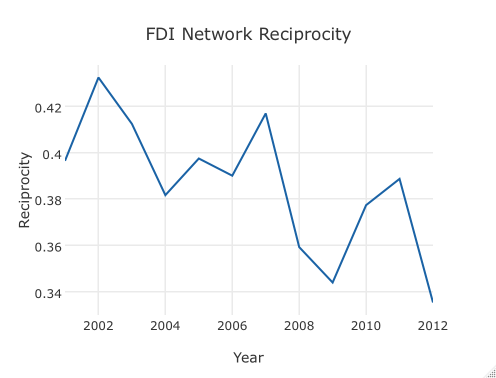
\includegraphics[scale=.8]{draft_figures/reciprocity.png}\\
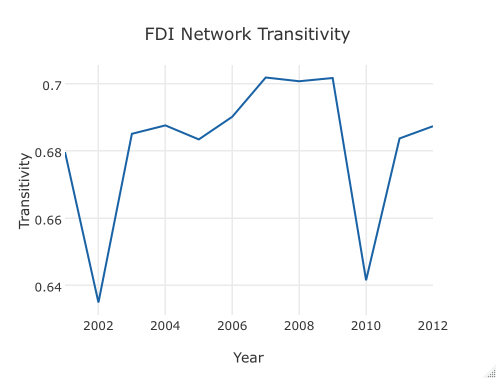
\includegraphics[scale=.8]{draft_figures/transitivity.png}\\
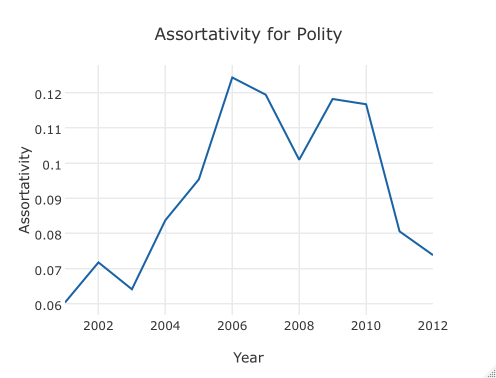
\includegraphics[scale=.8]{draft_figures/assortativity.png}\\
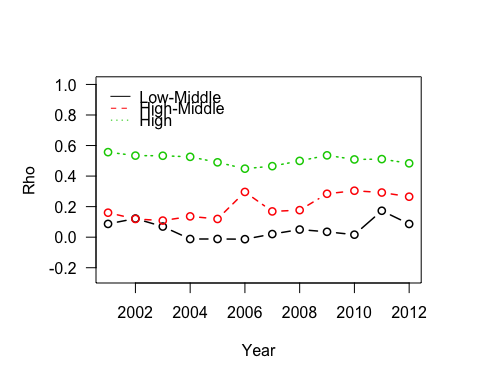
\includegraphics[scale=.8]{draft_figures/rho_income.png}\\
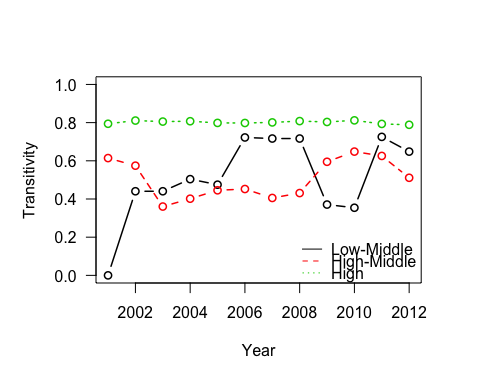
\includegraphics[scale=.8]{draft_figures/trans_income.png}\\
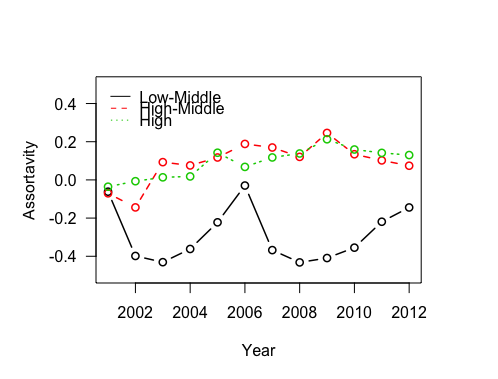
\includegraphics[scale=.8]{draft_figures/assort_income.png}

\subsection{Covariates}

We control for both economic and political variables. Following the literature's standard for predicting FDI inflows we include standard gravity variables. This includes the log product of the dyad's GDP and logged euclidean distance. Generally, larger products of GDP are associated with higher levels of FDI while longer distances are associated with less FDI \citep{mayer2011notes, WB1}. \\

The other key economic variable that is included trade in intermediate goods \citep{OECD}. This is constructed according to the UN Broad Economic Category classification definitions that separates goods by end-use category. Intermediate goods include unprocessed and partially processed agricultural goods and industrial goods. Past research has shown that FDI and trade are compliments \citep{aizenman2006fdi} and the advantage of using trade in intermediate goods is that it proxies for production supply chains, which we expect to be strongly positively associated with FDI inflows.\\

A more minor economic variable included is the growth rate of the economy, which has been used in past studies to stand in for the general health of a country's economy \citep{WB2}.\\

We include two categories of international agreement variables. The first is dummy variables for defense agreements \citep{Gibler09}. This includes defense, entente, non-aggression, and neutrality treaties. We expect these variables to positively associated with FDI inflows, particularly defense treaties since this indicates political cooperation and a lower risk of expropriation. The second international agreement variable is preferential trade agreement (PTA) depth \citep{dur2014design}. Past work has argued that PTAs represent a commitment to liberal markets that investors would favor and therefore would be associated with increased FDI inflows \citep{buthe2014foreign}. However, this study used monadic data and only a count PTAs signed. Our work takes this further since we are using network data and increases in PTA depth and FDI inflows is measured at the dyadic level and the PTA variable we use is built using latent trait analysis with 48 different variables.\\

There is substantial amount of work that explores the relationship between regime type and FDI inflows. The work is inconclusive, but include controls for it nonetheless using the Polity IV score \citep{polity2012polity}. We also include political violence to proxy for state stability, which expect to be negatively correlated with FDI inflows \citep{marshall2005major}.
\newpage
\subsection{Covariate Summary Statistics}

% Table created by stargazer v.5.2 by Marek Hlavac, Harvard University. E-mail: hlavac at fas.harvard.edu
% Date and time: Mon, Feb 20, 2017 - 22:08:59
\begin{table}[!htbp] \centering 
  \caption{} 
  \label{} 
\begin{tabular}{@{\extracolsep{5pt}}lccccc} 
\\[-1.8ex]\hline 
\hline \\[-1.8ex] 
Statistic & \multicolumn{1}{c}{N} & \multicolumn{1}{c}{Mean} & \multicolumn{1}{c}{St. Dev.} & \multicolumn{1}{c}{Min} & \multicolumn{1}{c}{Max} \\ 
\hline \\[-1.8ex] 
contig & 189,000 & 0.024 & 0.152 & 0 & 1 \\ 
comlang\_off & 189,000 & 0.112 & 0.315 & 0 & 1 \\ 
comlang\_ethno & 189,000 & 0.115 & 0.318 & 0 & 1 \\ 
colony & 189,000 & 0.015 & 0.121 & 0 & 1 \\ 
comcol & 189,000 & 0.062 & 0.241 & 0 & 1 \\ 
curcol & 189,000 & 0.0003 & 0.016 & 0 & 1 \\  
Defense Treaty & 189,000 & 0.075 & 0.264 & 0 & 1 \\ 
Non-aggression Treaty & 189,000 & 0.064 & 0.245 & 0 & 1 \\ 
Neutrality Treaty & 189,000 & 0.004 & 0.063 & 0 & 1 \\ 
Entente Treaty & 189,000 & 0.066 & 0.248 & 0 & 1 \\ 
\hline \\[-1.8ex] 
\end{tabular} 
\end{table} 



\newpage
\section{Results}
\begin{table}[!htbp] 
\begin{center}
\begin{tabular}{l c c }
\hline
 & Model 1 & Model 2 \\
\hline
sum                           & $2.21^{***}$  & $-1.52^{***}$ \\
                              & $(0.07)$      & $(0.16)$      \\
sum0.5                        & $-4.37^{***}$ & $0.47$        \\
                              & $(0.26)$      & $(0.30)$      \\
nonzero                       & $-1.72^{***}$ & $-4.52^{***}$ \\
                              & $(0.23)$      & $(0.24)$      \\
mutual.geom.mean              & $0.61^{***}$  & $-0.04$       \\
                              & $(0.03)$      & $(0.03)$      \\
edgecov.fdi\_net.mass.sum     &               & $0.18^{***}$  \\
                              &               & $(0.01)$      \\
edgecov.fdi\_net.distance.sum &               & $-0.24^{***}$ \\
                              &               & $(0.01)$      \\
\hline
AIC                           & -24739.37     & -27340.33     \\
BIC                           & -24708.71     & -27294.34     \\
Log Likelihood                & 12373.69      & 13676.17      \\
\hline
\multicolumn{3}{l}{\scriptsize{$^{***}p<0.001$, $^{**}p<0.01$, $^*p<0.05$}}
\end{tabular}
\caption{Statistical models for FDI Inflows}
\label{table:coefficients}
\end{center}
\end{table}

\begin{table}[!htbp] 
\begin{center}
\begin{tabular}{l c c }
\hline
 & Model 1 & Model 2 \\
\hline
sum                           & $2.37^{***}$  & $0.04$        \\
                              & $(0.05)$      & $(0.12)$      \\
sum0.5                        & $-4.14^{***}$ & $-0.67^{**}$  \\
                              & $(0.21)$      & $(0.25)$      \\
nonzero                       & $-2.55^{***}$ & $-6.17^{***}$ \\
                              & $(0.21)$      & $(0.27)$      \\
mutual.geom.mean              & $0.50^{***}$  & $0.02$        \\
                              & $(0.02)$      & $(0.02)$      \\
transitiveties                &               & $1.48^{***}$  \\
                              &               & $(0.16)$      \\
edgecov.fdi\_net.mass.sum     &               & $0.13^{***}$  \\
                              &               & $(0.00)$      \\
edgecov.fdi\_net.distance.sum &               & $-0.19^{***}$ \\
                              &               & $(0.01)$      \\
\hline
AIC                           & -29303.05     & -32432.34     \\
BIC                           & -29272.39     & -32378.69     \\
Log Likelihood                & 14655.53      & 16223.17      \\
\hline
\multicolumn{3}{l}{\scriptsize{$^{***}p<0.001$, $^{**}p<0.01$, $^*p<0.05$}}
\end{tabular}
\caption{Statistical models For FDI Stock}
\label{table:coefficients}
\end{center}
\end{table}

\begin{table}
\begin{center}
\begin{tabular}{l c c }
\hline
 & Model 1 & Model 2 \\
\hline
sum                              & $-0.98^{***}$ & $-0.61^{***}$ \\
                                 & $(0.15)$      & $(0.15)$      \\
sum0.5                           & $0.31$        & $-0.23$       \\
                                 & $(0.25)$      & $(0.24)$      \\
nonzero                          & $-5.25^{***}$ & $-6.26^{***}$ \\
                                 & $(0.24)$      & $(0.27)$      \\
edgecov.fdi\_net.mass.sum        & $0.15^{***}$  & $0.14^{***}$  \\
                                 & $(0.00)$      & $(0.00)$      \\
edgecov.fdi\_net.distance.sum    & $-0.21^{***}$ & $-0.20^{***}$ \\
                                 & $(0.01)$      & $(0.01)$      \\
edgecov.fdi\_net.contig.sum      & $-0.06$       & $-0.05$       \\
                                 & $(0.03)$      & $(0.03)$      \\
edgecov.fdi\_net.colony.sum      & $0.18^{***}$  & $0.16^{***}$  \\
                                 & $(0.03)$      & $(0.03)$      \\
edgecov.fdi\_net.lang\_ethno.sum & $0.09^{***}$  & $0.08^{***}$  \\
                                 & $(0.02)$      & $(0.02)$      \\
edgecov.fdi\_net.defence\_t.sum  & $0.10$        & $0.11$        \\
                                 & $(0.06)$      & $(0.07)$      \\
edgecov.fdi\_net.nonagg\_t.sum   & $-0.20^{**}$  & $-0.19^{**}$  \\
                                 & $(0.07)$      & $(0.06)$      \\
edgecov.fdi\_net.neut\_t.sum     & $0.20^{*}$    & $0.20^{*}$    \\
                                 & $(0.08)$      & $(0.08)$      \\
edgecov.fdi\_net.entente\_t.sum  & $0.06$        & $0.05$        \\
                                 & $(0.08)$      & $(0.08)$      \\
edgecov.fdi\_net.depth.sum       & $-0.02^{*}$   & $-0.02^{**}$  \\
                                 & $(0.01)$      & $(0.01)$      \\
nodeicov.sum..Polity             & $0.03^{***}$  & $0.03^{***}$  \\
                                 & $(0.00)$      & $(0.00)$      \\
nodeicov.sum..TradeOpen          & $0.00^{***}$  & $0.00^{***}$  \\
                                 & $(0.00)$      & $(0.00)$      \\
nodeicov.sum..GDP.g              & $-0.02^{***}$ & $-0.01^{***}$ \\
                                 & $(0.00)$      & $(0.00)$      \\
nodeicov.sum..PV                 & $-0.02^{**}$  & $-0.02^{**}$  \\
                                 & $(0.01)$      & $(0.01)$      \\
mutual.geom.mean                 &               & $0.02$        \\
                                 &               & $(0.02)$      \\
transitiveties                   &               & $1.42^{***}$  \\
                                 &               & $(0.17)$      \\
\hline
AIC                              & -33007.70     & -33129.09     \\
BIC                              & -32877.40     & -32983.46     \\
Log Likelihood                   & 16520.85      & 16583.54      \\
\hline
\multicolumn{3}{l}{\scriptsize{$^{***}p<0.001$, $^{**}p<0.01$, $^*p<0.05$}}
\end{tabular}
\caption{Statistical models}
\label{table:coefficients}
\end{center}
\end{table}




\section{Conclusion}


\newpage
\bibliographystyle{apsr}
\bibliography{fdi_reference}


\end{document}